\documentclass{standalone}
\usepackage{tikz}
\usepackage{pgf-umlcd}
\usepackage{fontspec,xcolor,ifthen,xifthen,textcomp}

\setmonofont[
    AutoFakeSlant,
    BoldItalicFeatures={FakeSlant},
]{Inconsolatazi4}

\newcommand{\fieldType}[2]{\texttt{\color{red}{#1:\hspace{1mm}#2}}}
\newcommand{\funcType}[4][]{\texttt{\color{blue}{#2(#3)%
    \ifthenelse{\isempty{#4}}%
    {}%
    {\hspace{1mm}#4}%
    \ifthenelse{\isempty{#1}}%
    {}%
    {:\hspace{1mm}#1}%
}}}

\begin{document}

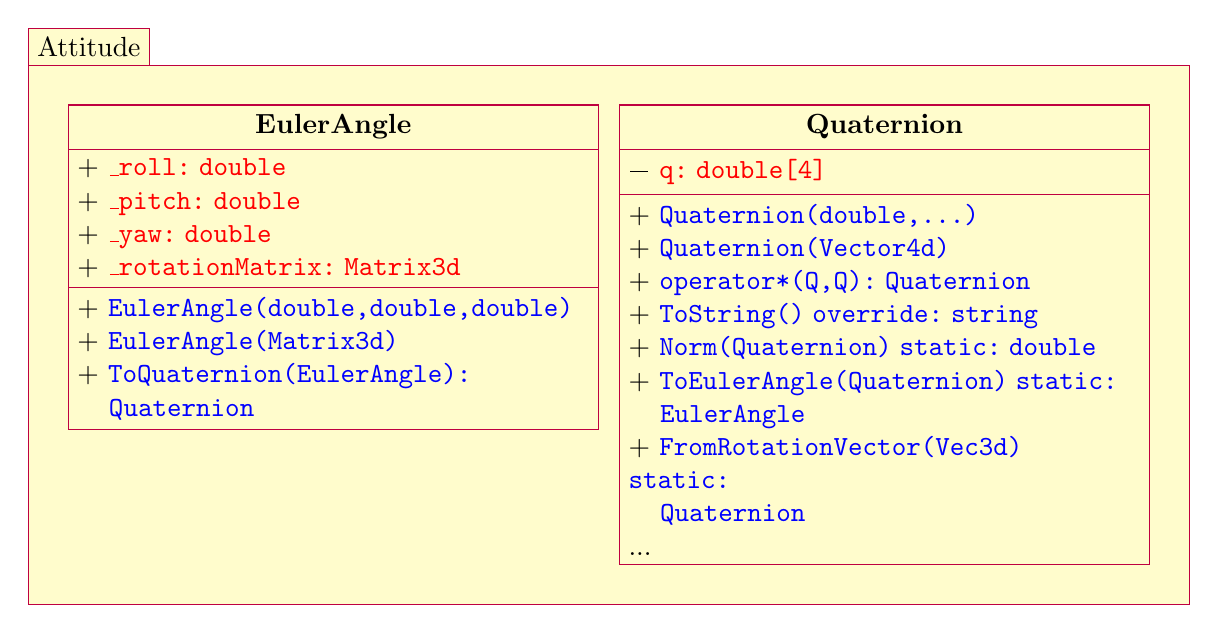
\begin{tikzpicture}
\begin{package}{Attitude}
\begin{class}[text width =6.5cm]{EulerAngle}{-3.5 , 0}
\attribute{+ \fieldType{\_roll}{double}}
\attribute{+ \fieldType{\_pitch}{double}}
\attribute{+ \fieldType{\_yaw}{double}}
\attribute{+ \fieldType{\_rotationMatrix}{Matrix3d}}
\operation{+ \funcType{EulerAngle}{double,double,double}{}}
\operation{+ \funcType{EulerAngle}{Matrix3d}{}}
\operation{+ \funcType[\\ \phantom{+ }\hspace{1mm}Quaternion]{ToQuaternion}{EulerAngle}{}}
\end{class}
\begin{class}[text width =6.5 cm]{Quaternion}{3.5 , 0}
\attribute{\textminus\phantom{ }\fieldType{q}{double[4]}}
\operation{+ \funcType{Quaternion}{double,...}{}}
\operation{+ \funcType{Quaternion}{Vector4d}{}}
\operation{+ \funcType[Quaternion]{operator*}{Q,Q}{}}
\operation{+ \funcType[string]{ToString}{}{override}}
\operation{+ \funcType[double]{Norm}{Quaternion}{static}}
\operation{+ \funcType[\\ \phantom{+ }\hspace{1mm}EulerAngle]{ToEulerAngle}{Quaternion}{static}}
\operation{+ \funcType[\\ \phantom{+ }\hspace{1mm}Quaternion]{FromRotationVector}{Vec3d}{static}}
\operation{...}
\end{class}
\end{package}
\end{tikzpicture}

\end{document}